% This file demonstrates how to use the IEEEConf LaTeX2e macro package,
% to prepare a manuscript for proceedings on CD of the conference
% FedCSIS
%
\documentclass[conference]{IEEEtran}
%\documentclass[a4paper]{IEEEconf}

% This package serves to balance the column lengths on the last page of the document.
% please, insert \balance command in the left column of the last page
\usepackage{balance}

%% to enable \thank command
\IEEEoverridecommandlockouts 
%% The usage of the following packages is recommended
%% to insert graphics
\usepackage[dvips]{graphicx}
% to typeset algorithms
\usepackage{algorithmic}
\usepackage{algorithm}
% to typeset code fragments
\usepackage{listings}
% to make an accent \k be available
\usepackage[OT4,T1]{fontenc}
% provides various features to facilitate writing math formulas and to improve the typographical quality of their output.
\usepackage[cmex10]{amsmath}
\interdisplaylinepenalty=2500
% por urls typesetting and breaking
\usepackage{url}
% for vertical merging table cells
\usepackage{multirow}

% define environments for remarks and examples
\newtheorem{remark}{Remark}[section]
\newtheorem{example}[remark]{Example}


%
%
\title{How to Use the IEEEtran Macro Package for Preparing a Manuscript for the FedCSIS e-Proceedings\thanks{This work was not supported by any organization}}
%
%
\author{
\IEEEauthorblockN{Aleksander Denisiuk}
\IEEEauthorblockA{
University of Warmia and Mazury\\
in Olsztyn\\
ul.\ S{\l}oneczna 54, 10-710 Olsztyn, Poland\\
Email: denisjuk@matman.uwm.edu.pl}
\and
\IEEEauthorblockN{Second Author, Third Author}
\IEEEauthorblockA{Universit\'{e} de Paris-Sud,\\
Laboratoire d'Analyse Num\'{e}rique,\\
B\^{a}timent 425,\\
F-91405 Orsay Cedex, France\\
Email: \{second, third\}@subdomain.domain.fr}
}

% conference papers do not typically use \thanks and this command
% is locked out in conference mode. If really needed, such as for
% the acknowledgment of grants, issue a \IEEEoverridecommandlockouts
% after \documentclass

% for over three affiliations, or if they all won't fit within the width
% of the page, use this alternative format:
% 
%\author{\IEEEauthorblockN{Michael Shell\IEEEauthorrefmark{1},
%Homer Simpson\IEEEauthorrefmark{2},
%James Kirk\IEEEauthorrefmark{3}, 
%Montgomery Scott\IEEEauthorrefmark{3} and
%Eldon Tyrell\IEEEauthorrefmark{4}}
%\IEEEauthorblockA{\IEEEauthorrefmark{1}School of Electrical and Computer Engineering\\
%Georgia Institute of Technology,
%Atlanta, Georgia 30332--0250\\ Email: see http://www.michaelshell.org/contact.html}
%\IEEEauthorblockA{\IEEEauthorrefmark{2}Twentieth Century Fox, Springfield, USA\\
%Email: homer@thesimpsons.com}
%\IEEEauthorblockA{\IEEEauthorrefmark{3}Starfleet Academy, San Francisco, California 96678-2391\\
%Telephone: (800) 555--1212, Fax: (888) 555--1212}
%\IEEEauthorblockA{\IEEEauthorrefmark{4}Tyrell Inc., 123 Replicant Street, Los Angeles, California 90210--4321}}





\begin{document}
\maketitle              % typeset the title of the contribution

\begin{abstract}
This document describes the rules one should follow to prepare the article for the FedCSIS e-proceedings
The abstract may be up to 150 words.
\end{abstract}


\section{Introduction}
%
\IEEEoverridecommandlockouts\IEEEPARstart{T}{o prepare} the article for the FedCSIS \hbox{e-}pro\-cee\-dings, please use the IEEEtran \LaTeXe\ macro package (document class \verb|IEEEtran|). This document contains some hints how to use certain \LaTeX\ packages to fit the conference proceedings format. You can use the source of this document as a template for typesetting of your paper.
\subsection{For Beginners}
For \LaTeX\ beginners I would like to recommend  to visit the site of the \TeX\ Users Group and, specifically the book ``The Not So Short Introduction to \LaTeXe,'' by Tobias Oetiker:
\url{http://www.tug.org/begin.html}
\begin{remark}
Using \LaTeXe\ macros authors should define only the \emph{logical structure} of the text. You are not allowed to use macros that explicitly change fonts, break lines, pages. etc.
\end{remark}

\subsection{Macros downloading}
%
The IEEEconf \LaTeXe\ macro package can be downloaded from CTAN: \url{http://www.ctan.org/tex-archive/macros/latex/contrib/IEEEconf/}
as well as from the conference site.
The conference cite contains also the last version of this document and its source.
\section{Preamble}

\subsection{Paper size}
Please, indicate in the preamble a4 paper size in the following way:
\begin{verbatim}
\documentclass[a4paper, conference]
    {IEEEtran}
\end{verbatim}

\subsection{Polish accent ``ogonek''}
To make the polish accent {\k \ } (``ogonek'') available use package \verb|fontenc| with the option \verb|OT4,T1|
\begin{verbatim}
\usepackage[OT4,T1]{fontenc}
\end{verbatim}

\subsection{Initial Drop Cap Letter}
 The first letter of a journal paper is a large, capital, oversized
letter which descends one line below the baseline. Such a
letter is called a ``drop cap'' letter. The other letters in the first
word are rendered in upper case. This effect can be accurately
produced using the IEEEtran command \verb|\IEEEPARstart{}{}|. The first argument is the first letter of the first word, the
second argument contains the remaining letters of the first
word. The drop cap of this document was produced with:
$$\verb|\IEEEPARstart{W}{ith}|$$

Note that the second word should also be rendered  in
upper case if the first word is very short (less than 3~letters):
$$\verb|\IEEEPARstart{T}{o prepare}|$$


\section{Figures and Tables}
To insert a figure you are encouraged to use the  \verb|graphicx| package. Please, include this package in the preamble with the option \verb|dvips|:
\begin{verbatim}
\usepackage[dvips]{graphicx}
\end{verbatim}
Figures in the \verb|eps| format should be inserted in the \verb|figure| environment, as follows:
\begin{verbatim}
\begin{figure}[tbp]
\centering
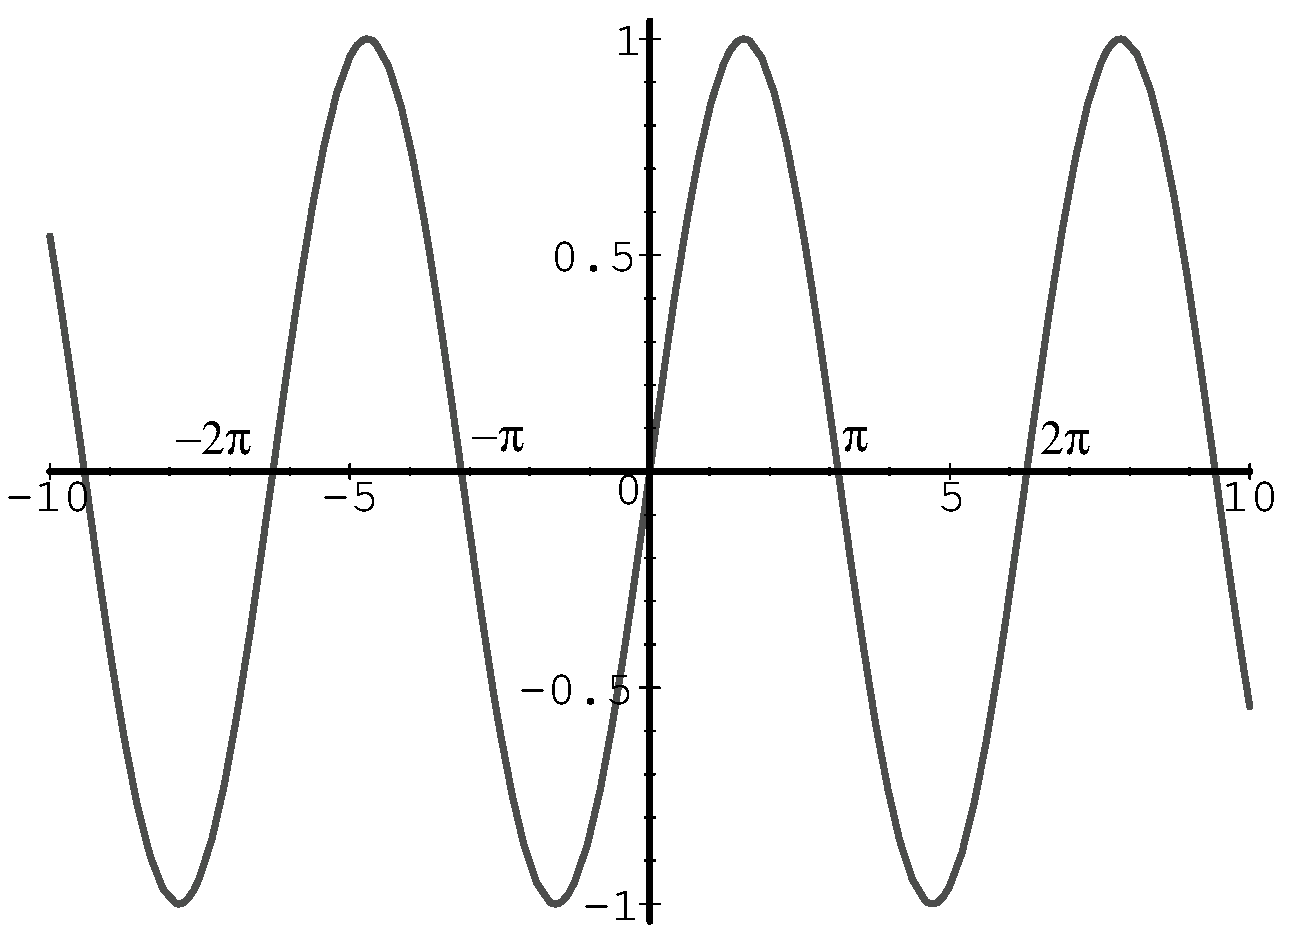
\includegraphics[width=0.75\hsize]
     {test.eps}
\caption{Sinusoid}
\end{figure}
\end{verbatim}
%
\begin{figure}[tbp]
\centering
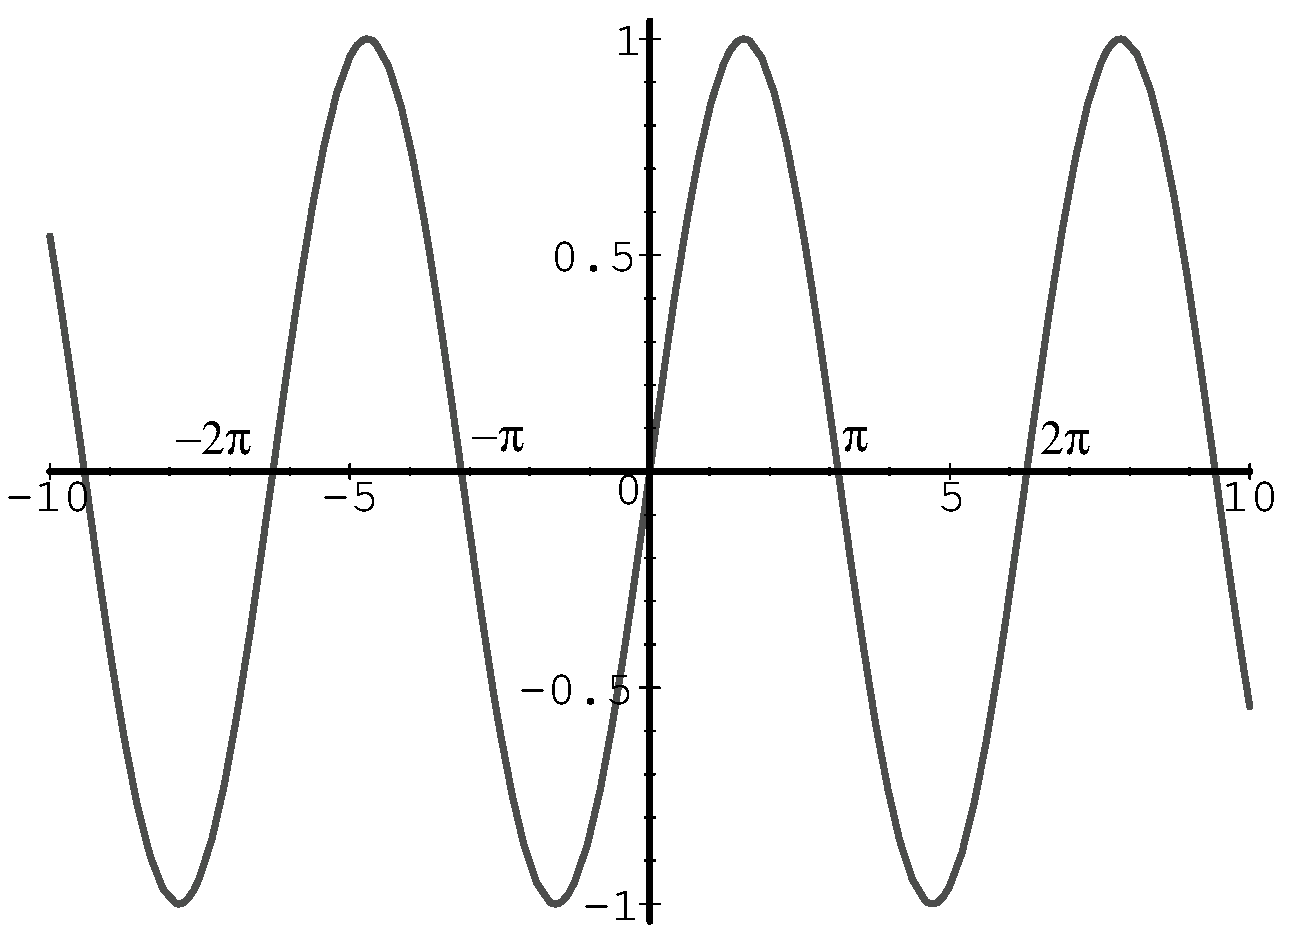
\includegraphics[width=0.75\hsize]{test.eps}
\caption{Sinusoid}
\end{figure}
%
Parameters of the command \verb|\includegraphics| are described in the documentation of the \verb|graphicx| package.

Prepare your figures using vector graphics and converting it to standard eps format (without Corel Draw extensions). Photo eps files should be obtained from high-resolution (at least 300 DPI) JPEG files. Consider using of \LaTeX\ packages (TeXDraw, XYpic, etc) for producing high-quality schemes and graphics. If your graphical editor is Microsoft Office, try to copy your Excell chart and paste it in OpenOffice Draw. Than use Export as EPS option.


Pay attention that the figure caption is placed \emph{below} the figure, while the table caption is placed \emph{above} the table (cf.~table~\ref{table}). Figures or tables may span both columns, if necessary (use \texttt{figure*} or \texttt{table*} environments).


\begin{table*}[tbp]
\caption{Defining characteristics of five early digital computers}\label{table}
\centering
\begin{tabular}{|@{\vrule width0ptheight9pt\enspace}l|c|c|c|c|c|c|c|}\hline
\hfil\bf Computer&\bf First operation&\bf Place& \bf Decimal/Binary&\bf Electronic&\bf Programmable&\bf Turing complete\\\hline
Zuse Z3&May 1941&Germany&binary&No&By punched film stock&Yes (1998)\\\hline
Atanasoff-Berry Computer&Summer 1941&USA&binary&Yes&No&No\\\hline
Colossus&1943--1944&UK&binary&Yes&Partially, by rewiring&No\\\hline
Harvard Mark I--IBM ASCC&1944&USA&decimal&No&By punched paper tape&Yes (1998)\\\hline
\multirow{2}{*}{ENIAC}&1944&USA&decimal&Yes&Partially, by rewiring&Yes\\\cline{2-7}
&1948&USA&decimal&Yes&By Function Table ROM&Yes\\\hline
\end{tabular}
\end{table*}

Position figures and tables at the tops and bottoms of columns.  Avoid placing them in the middle of columns.  Large figures and tables my span across both columns.  Figure captions should be below the figures; table captions should be above the tables.  Avoid placing figures and tables before their first mention in the text.  Use the abbreviation ``Fig.~1,'' even at the beginning of a sentence.


\section{Algorithms}

For algorithms typesetting the packages \verb|algorithmic| and~\verb|algorithm| are used. 

The first one defines environment \verb|algorithmic|, inside which algorithms are inputted. In the following example the code from the left side produces the output shown on the right side. The optional parameter~\verb|[2]| defines lines numeration of the algorithm.

The  package \verb|algorithm| defines new float environment \verb|algorithm| which is  similar to floats \verb|figure| and \verb|table|. 

The usage of the \verb|algorithm| environment is presented in the example~\ref{algorytm}, output---algorithm~\ref{example}---is respectively given on the page~\pageref{example}.


\begin{example}[the \texttt{algorithm} environment]\label{algorytm}
Coding:\begin{verbatim}\begin{algorithm}[tbp]
\caption{Calculating $x$ to the 
power~$n$\label{example}}
\begin{algorithmic}[2]
\REQUIRE $n\ge 0$
\ENSURE $a=x^n$
\STATE $k\leftarrow n$; $a\leftarrow 1$; 
\STATE $b\leftarrow x$;
\WHILE[Invariant: $x^n=a\cdot b^k$]
{$k>0$}
\IF{$k$ is even}
\STATE $k\leftarrow k/2$;
\STATE $b\leftarrow b\cdot b$;
\ELSE[$k$ is odd]
\STATE $k\leftarrow k-1$;
\STATE $a\leftarrow a\cdot b$;
\ENDIF
\ENDWHILE
\end{algorithmic}
\end{algorithm}
\end{verbatim}
\end{example}

Output is given on the page~\pageref{example}
\begin{algorithm}[tbp]
\caption{Calculating $x$ to the 
power~$n$\label{example}}
\begin{algorithmic}[2]
\REQUIRE $n\ge 0$
\ENSURE $a=x^n$
\STATE $k\leftarrow n$; $a\leftarrow 1$; 
\STATE $b\leftarrow x$;
\WHILE[Invariant: $x^n=a\cdot b^k$]
{$k>0$}
\IF{$k$ is even}
\STATE $k\leftarrow k/2$;
\STATE $b\leftarrow b\cdot b$;
\ELSE[$k$ is odd]
\STATE $k\leftarrow k-1$;
\STATE $a\leftarrow a\cdot b$;
\ENDIF
\ENDWHILE
\end{algorithmic}
\end{algorithm}


\section{Code fragments}
To include the programming code fragment, please use the package \verb|listings|. This package ``understands'' almost all the programming languages and their dialects from BASIC to XML. Particulars of the package usage are given in the package documentation. In what follows we show implementations of the algorithm~\ref{example} in C++. Examples contain \TeX-code and the corresponding output.

\begin{example}[C++]
Coding:
\begin{verbatim}
\lstset{language=C++}
\begin{lstlisting}
int power(int x,int n){
   int k,a,b;
   k=n; a=1; b=x;
   while(k>0){//Invariant: x^n=a*b^k
      if (k % 2==0){
         k/=2;
         b*=b;
      }
      else{
         k--;
         a*=b;
      }
   }
   return a;
}
\end{lstlisting}
\end{verbatim}
Output is shown on the page~\pageref{c++}
\begin{algorithm}[tbp]
\caption{Calculating $x$ to the 
power~$n$ in C++\label{c++}}
\lstset{language=C++}
\begin{lstlisting}
int power(int x,int n){
   int k,a,b;
   k=n; a=1; b=x;
   while (k>0) {// Invariant: x^n=a*b^k
      if (k % 2==0){
         k/=2;
         b*=b;
      }
      else{
         k--;
         a*=b;
      }
   }
   return a;
}
\end{lstlisting}
\end{algorithm}
\end{example}



\section{References}
For bibliography references use the standard \LaTeX\ tools. Refer simply to the reference number, as in~\cite{c3}. Do not use ``Ref.~\cite{c3}'' or ``reference~\cite{c3}'' except at the beginning of a sentence:  ``Reference~\cite{c3} was the first\dots''. Do not put footnotes in the reference list. IEEE Transactions no longer use a journal prefix before the volume number.  For example, use ``IEEE Trans.\ Magn., vol.~25,'' not ``vol.~MAG-25.''

Give all authors' names; do not use ``et al.'' unless there are six authors or more.  Papers that have not been published, even if they have been submitted for publication, should be cited as ``unpublished'' \cite{cu}.  Papers that have been accepted for publication should be cited as ``in press'' \cite{cin}.  Capitalize only the first word in a paper title, except for proper nouns and element symbols.
For papers published in translation journals, please give the English citation first, followed by the original language citation~\cite{ctr}.

% serves to balance the column lengths on the last page of the document
% should be inserted the left column of the last page
\balance



\section{Some Common Mistakes}
The word ``data'' is plural, not singular.  In American English, periods and commas are within quotation marks, like ``this period.''  A parenthetical statement at the end of a sentence is punctuated outside of the closing parenthesis (like this).  (A parenthetical sentence is punctuated within the parentheses.)  A graph within a graph is an ``inset,'' not an ``insert.''  The word alternatively is preferred to the word ``alternately'' (unless you really mean something that alternates).  Do not use the word ``essentially'' to mean ``approximately'' or ``effectively.''  Be aware of the different meanings of the homophones ``affect'' and ``effect,'' ``complement'' and ``compliment,'' ``discreet'' and ``discrete,'' ``principal'' and ``principle.''  Do not confuse ``imply'' and ``infer.''  The prefix ``non'' is not a word; it should be joined to the word it modifies, usually without a hyphen.  There is no period after the ``et'' in the Latin abbreviation ``et al.''  The abbreviation ``i.e.'' means ``that is,'' 
and the abbreviation ``e.g.'' means ``for example.'' Microsoft Office in not a~graphical editor. An excellent style manual and source of information for science writers is~\cite{c7}.

\section{Conclusion}
A conclusion section is not required. Although a conclusion may review the main points of the paper, do not replicate the abstract as the conclusion. A conclusion might elaborate on the importance of the work or suggest applications and extensions. 

\section{Submission}
Submitting the article, please, provide
\begin{itemize}
\item The source of the article.
\item Files of all the inserted graphics.
\item PDF file with the article. PDF will be sent to the referees.
\end{itemize}

\section*{Appendix}
Appendixes, if needed, appear before the acknowledgment.

\section*{Acknowledgment}
The preferred spelling of the word ``acknowledgment'' in America is without an ``e'' after the ``g.''  Try to avoid the stilted expression, ``One of us (R.~B.~G.) thanks \dots'' Instead, try ``R.~B.~G.\ thanks\dots''  Put sponsor acknowledgments in the unnumbered footnote on the first page.


\begin{thebibliography}{99}

\bibitem{c1}
J. G. F. Francis, ``The QR Transformation I,'' {\it Comput.\ J.,} vol.~4, 1961, pp.~265--271.

\bibitem{c2}
H. Kwakernaak and R. Sivan, {\it Modern Signals and Systems,} Prentice Hall, Englewood Cliffs, NJ; 1991.

\bibitem{c3}
D. Boley and R. Maier, ``A Parallel QR Algorithm for the Non-Symmetric Eigenvalue Algorithm,'' {\it in Third SIAM Conference on Applied Linear Algebra,} Madison, WI, 1988, pp.~A20.


\bibitem{c7}
M. Young, {\it The Technical Writer's Handbook.} Mill Valley, CA:  University Science, 1989.

\bibitem{cg}
IEEE Guidelines for Author
Supplied Electronic
Text and Graphics, \url{http://www.ieee.org/portal/cms_docs_iportals/iportals/publications/journmag/transactions/eic-guide.pdf}

\bibitem{cu} K. Elissa, ``Title of paper if known,'' unpublished.
\bibitem{cin} ``R. Nicole, Title of paper with only first word capitalized,'' J.\ Name Stand.\ Abbrev., in press.
\bibitem{ctr} Y. Yorozu, M. Hirano, K. Oka, and Y. Tagawa, ``Electron spectroscopy studies on magneto-optical media and plastic substrate interface,'' IEEE Transl.\ J.\ Magn.\ Japan, vol.~2, pp.~740--741, August 1987 [Digests 9th Annual Conf. Magnetics Japan, p.~301, 1982].

\end{thebibliography}


\end{document}
